\chapter{Introduction}\label{chapter-1-introduction}

\section{Overview}\label{10-overview}

This chapter motivates the design of SimForge, a reproducible
cross-simulator testing framework for urban mobility simulation. It
opens with the practical importance of traffic-simulation outputs in
transportation planning and policy, surveys the structural barriers that
have prevented fair cross-simulator comparison to date, declares the
research questions the thesis answers, summarizes the contributions, and
outlines how the remaining chapters are organized.

The central premise: although individual urban-mobility simulators
(SUMO, MATSim, DTALite, and others) are mature, the question
\emph{"which simulator should I trust for this planning decision?"} has
no defensible answer without a framework that runs them under identical
inputs, identical execution policies, and a programmatic audit that
verifies fairness. SimForge provides that framework, and the empirical
findings that emerged from building it are themselves contributions to
the cross-simulator benchmarking literature.

\begin{center}\rule{0.5\linewidth}{0.5pt}\end{center}

\section{Motivation}\label{11-motivation}

Urban transportation simulation is the empirical backbone of modern
infrastructure planning. Departments of transportation, regional
planning organizations, and academic research groups use traffic
microsimulation and mesoscopic flow models to evaluate congestion-
pricing schemes, infrastructure investments, traffic-signal-
coordination strategies, transit-priority interventions, and
emergency-evacuation plans. The simulators that produce these
evaluations --- SUMO (Eclipse, 2002--present), MATSim (ETH Zürich

\begin{itemize}
\tightlist
\item
  TU Berlin, 2008--present), POLARIS (Argonne National Laboratory,
  2014--present), DTALite (Arizona State University, 2010--present), and
  others --- each represent decades of accumulated modeling expertise,
  calibration practice, and operational tooling.
\end{itemize}

Despite this maturity, a foundational methodological problem remains:
\emph{which simulator\textquotesingle s output should a practitioner
trust on a given scenario?} Each simulator embodies different modeling
assumptions, uses different input formats, runs under different
execution conventions, and reports different metric definitions. A 10 \%
difference in mean travel time between SUMO and MATSim on the same
nominal scenario could plausibly reflect:

\begin{enumerate}
\def\labelenumi{\arabic{enumi}.}
\tightlist
\item
  A genuine paradigm-level modeling disagreement,
\item
  A subtle difference in how each engine interpreted the input,
\item
  A difference in how each engine\textquotesingle s developer tuned
  defaults,
\item
  A non-deterministic floating-point or threading effect,
\item
  An undocumented version mismatch between two installations.
\end{enumerate}

Practitioners who must choose a tool for an actual planning decision
have no operational way to distinguish (1) from (2)-(5), because the
published cross-simulator comparison literature does not typically
isolate them. The decision becomes a function of which simulator the
practitioner is already familiar with, which is not the basis on which
infrastructure investments worth billions of dollars per year should be
made.

The methodological gap is well-documented. Surveys of agent-based
transportation modeling have flagged it consistently \cite{bazzan2014review}; computational-reproducibility studies in adjacent
fields (machine learning \cite{pineau2021reproducibility}, computational biology
\cite{goodman2016reproducibility}) have identified the same pattern of
version-pinning insufficiency that this thesis measures empirically for
transportation simulation in Chapter 5 §5.6.3. The MLPerf benchmark
suite has demonstrated in machine learning that standardized cross-tool
benchmarks accelerate field progress; no equivalent framework existed
for urban-mobility simulation at the time the plan for this thesis
was submitted (December 2025).

\begin{center}\rule{0.5\linewidth}{0.5pt}\end{center}

\section{Problem statement}\label{12-problem-statement}

The central problem this thesis addresses is the absence of an
\emph{open, reproducible, simulator-neutral framework} that enables fair
cross-simulator comparison for urban-mobility simulation under
controlled, hash-pinned, hardware-normalized conditions. More
specifically:

\begin{enumerate}
\def\labelenumi{\arabic{enumi}.}
\item
  \textbf{No canonical input bundle.} Each simulator (SUMO, MATSim,
  DTALite, ...) consumes its own native input format (\texttt{.net.xml}
  + \texttt{.rou.xml} for SUMO; \texttt{network.xml} +
  \texttt{plans.xml} for MATSim; GMNS-format CSVs for DTALite). A
  cross-simulator comparison that does not normalize the input layer
  cannot distinguish input-interpretation differences from
  engine-behavior differences.
\item
  \textbf{No deterministic adapter chain.} Each simulator has its own
  sources of non-determinism (random seeds, thread scheduling,
  floating-point ordering). Without explicit deterministic-execution
  wrappers, repeated runs of the same simulator on the same input can
  produce different outputs, and the cross-simulator comparison becomes
  a comparison of distributions rather than of paradigms.
\item
  \textbf{No programmatic fairness audit.} Even when canonical inputs
  and deterministic adapters are in place, a reader of cross- simulator
  results has no way to verify the fairness claim without inspecting
  each engine\textquotesingle s input files manually. A
  machine-checkable audit is required.
\item
  \textbf{No pinned-digest execution environment.} Even with all of the
  above in place, the engines themselves depend on platform-specific
  binaries (SUMO is compiled per-OS; MATSim runs on a JVM whose build
  affects floating-point output; DTALite\textquotesingle s bundled
  binary uses an OpenMP runtime whose version affects parallel-reduction
  ordering). Without a pinned-digest container, "same version" does not
  guarantee "same output", and the cross-simulator benchmark becomes
  platform-bound rather than algorithm-bound.
\end{enumerate}

The thesis problem is therefore: \textbf{build a framework that closes
all four gaps}, then use it to make empirical measurements that
demonstrate the framework\textquotesingle s claims and surface findings
the framework makes newly visible.

\begin{center}\rule{0.5\linewidth}{0.5pt}\end{center}

\section{Research questions}\label{13-research-questions}

The thesis is structured around four research questions, restated from
the original December 2025 plan §1.12 and refined as the work
progressed:

\textbf{RQ1 (Fidelity).} Under identical canonical inputs and identical
execution policies, how closely do different simulation engines
reproduce \emph{each other\textquotesingle s} outputs on the same
scenario? The plan originally posed this question against
observed-baseline data (RMSE, GEH, KS vs sensor measurements). As
discussed in Chapter 6 §6.4.1, the shipped framework substitutes
\emph{inter-engine} fidelity (Chapter 5 §5.3, §5.6.2) for
fidelity-vs-reality, because the observed-baseline data integration was
scoped out for compute budget reasons.

\textbf{RQ2 (Scalability).} How does engine runtime scale with agent
count, network size, and execution-context (host venv vs pinned-digest
container), once normalized per-core? The plan also asked for
per-watt normalization; this was dropped because HPC environments do not
expose live power meters at the job allocation level. Chapter 5 §5.1 and
§5.5, and Chapter 6 §6.2.1 report the scalability results.

\textbf{RQ3 (Reproducibility).} Under fixed seeds, deterministic
adapters, and pinned-digest containers, what level of run-to-run output
variance remains? The thesis measures R = 1 − σ/μ on travel-time means
across repeated runs (Chapter 5 §5.2). The shipped framework achieves R
= 1.0000 for MATSim and DTALite within a fixed execution context, and R
≥ 0.95 for SUMO across all shipped cells. A novel sub-finding (Chapter 5
§5.6.3, Chapter 6 §6.2.3): at fixed code, the framework is bit-identical
across every measured platform; the 0.2-3 \% shifts originally reported
in cross-platform comparisons are code-version drift, not platform
drift.

\textbf{RQ4 (Trade-offs).} What fidelity-throughput-paradigm trade-offs
emerge across simulators, and are these trade-offs stable across urban
topologies, congestion regimes, and computational architectures? Chapter
5 §5.4 (micro vs meso within SUMO) and §5.6.2 (meso vs meso across SUMO
and MATSim at saturation density) report two distinct trade-off regimes.
The cross-engine ratio is shown to be regime-dependent, not
regime-stable, and the saturation regime is where the paradigm signal
becomes sharpest.

\begin{center}\rule{0.5\linewidth}{0.5pt}\end{center}

\section{Contributions}\label{14-contributions}

This thesis delivers four principal contributions, corresponding to the
plan\textquotesingle s §1.11 C1-C4, and surfaces four empirical
findings that emerged during the build and form part of the
framework\textquotesingle s contribution beyond the original C-row list.

\pandocbounded{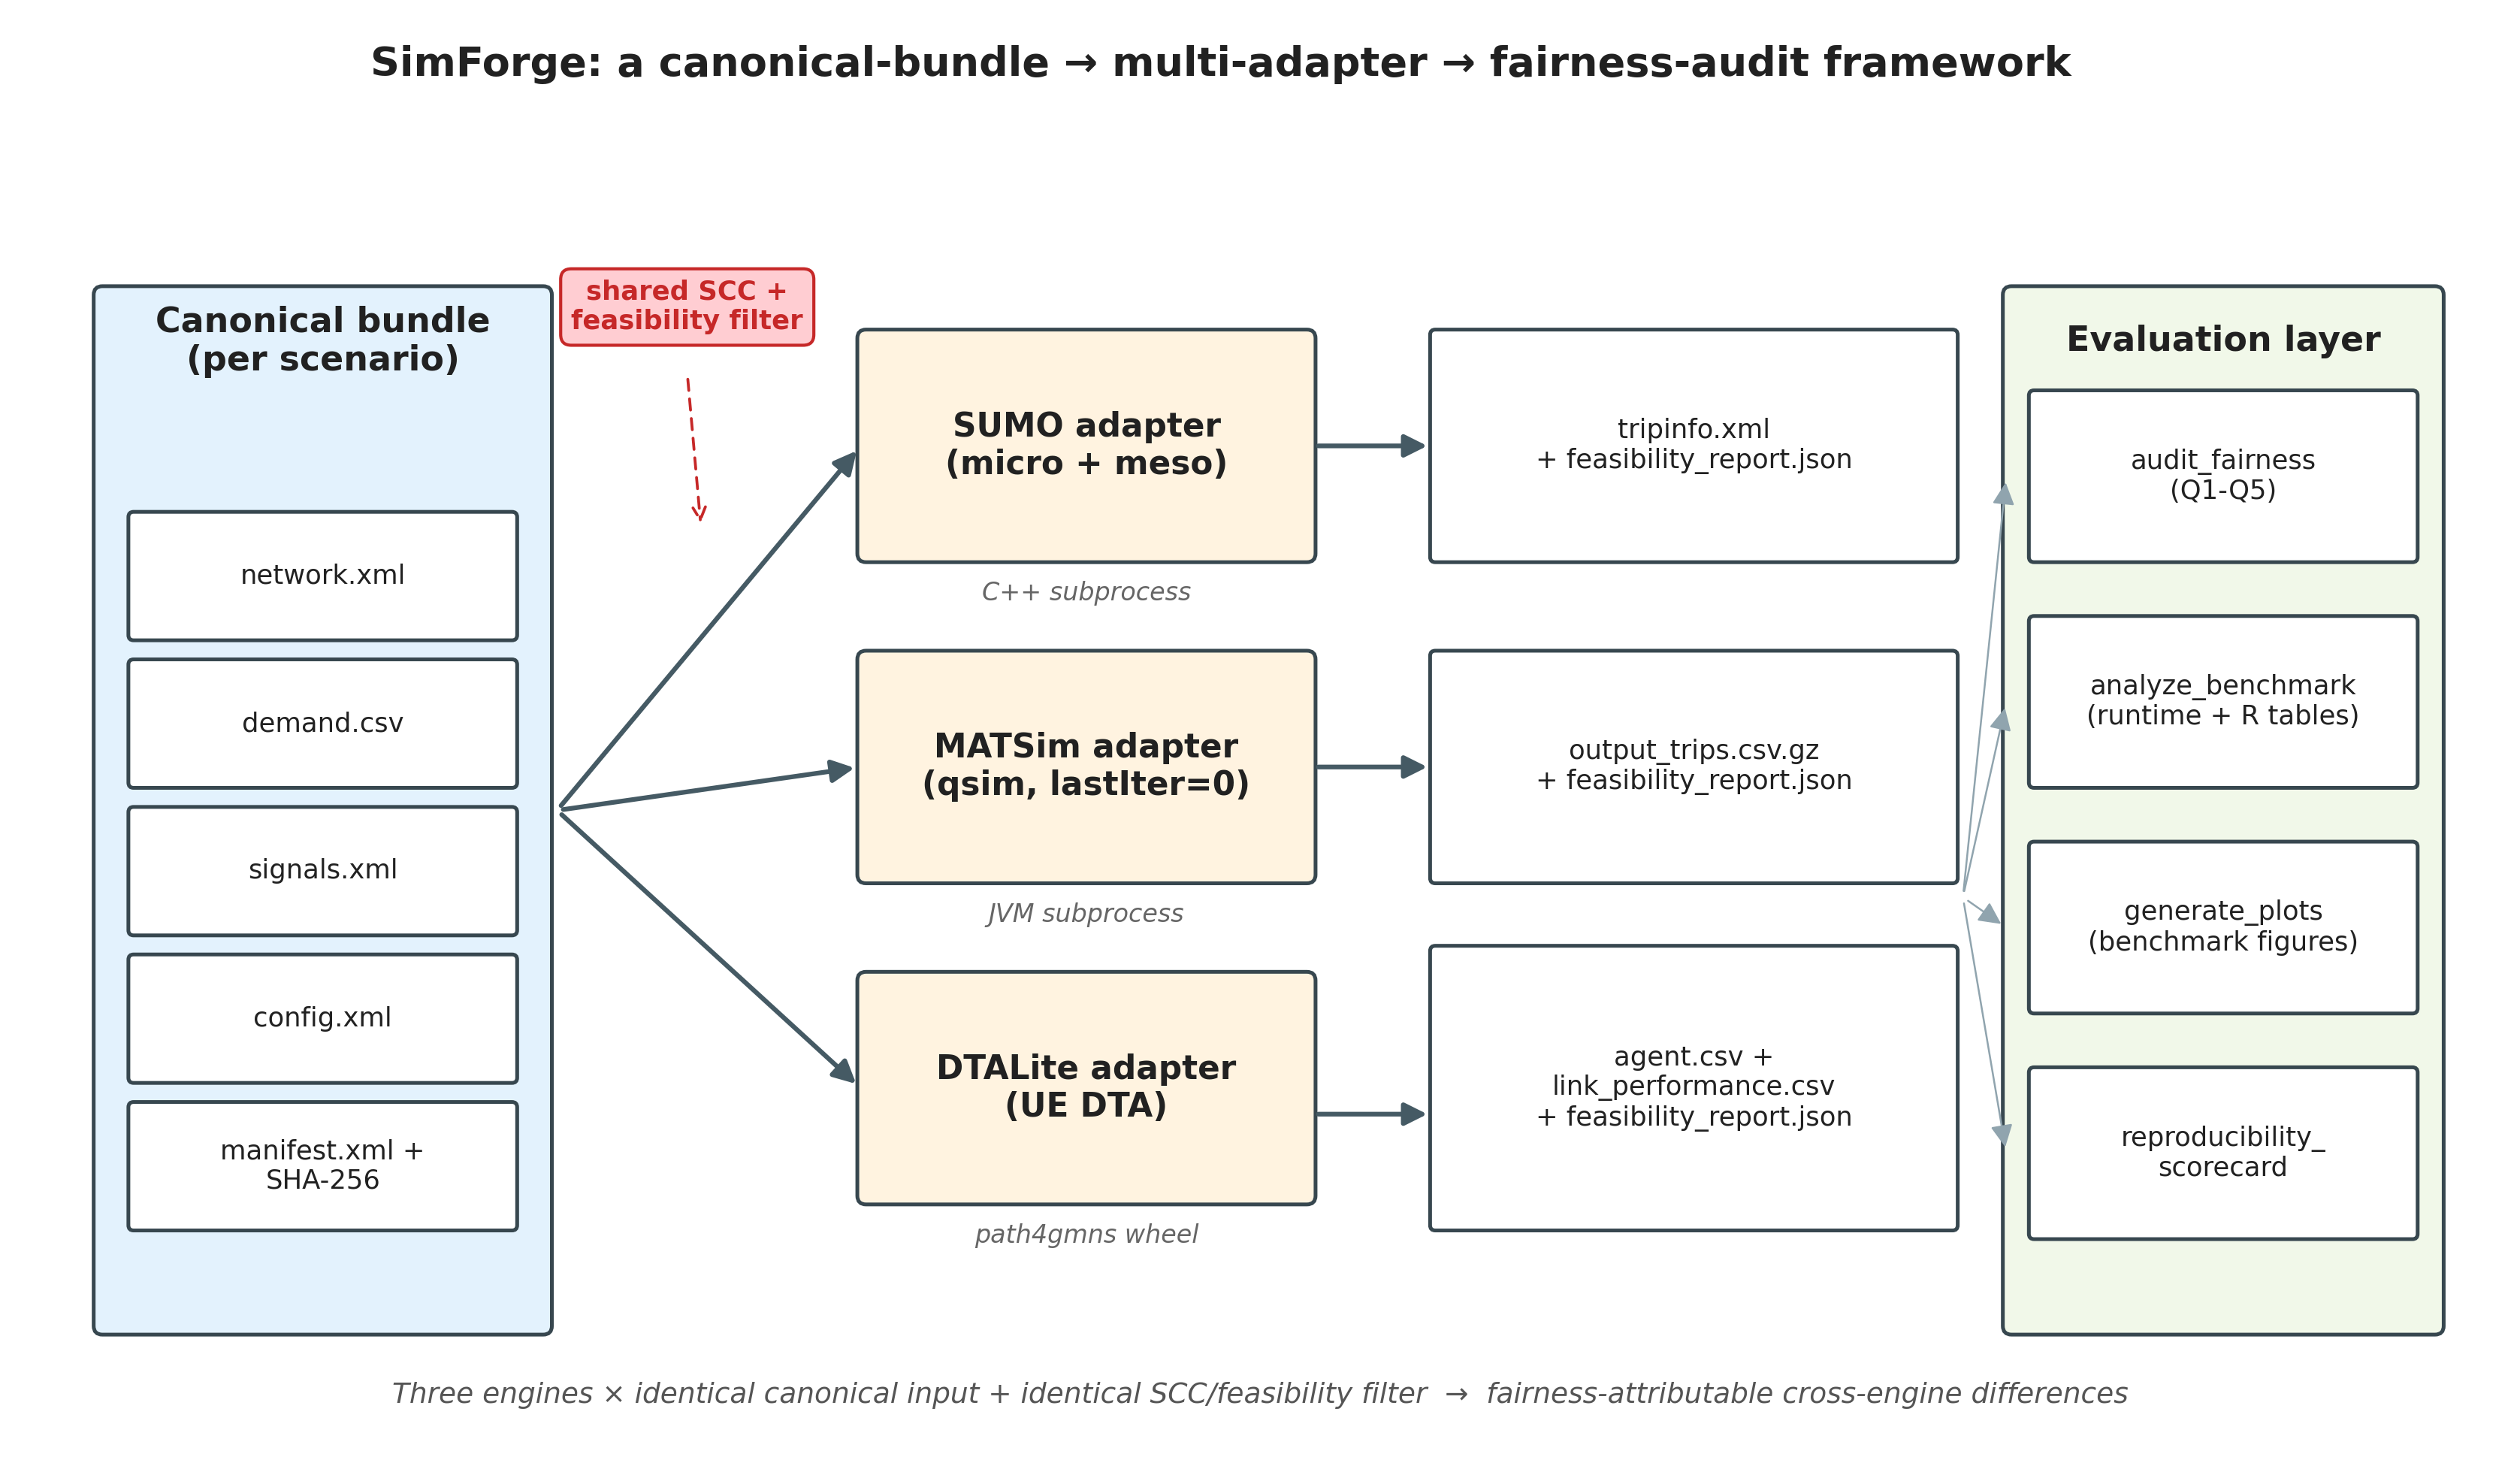
\includegraphics[keepaspectratio]{../figures/fig_1_1_simforge_overview.png}}

\subsection{The four delivered C-rows (per plan
§1.11)}\label{141-the-four-delivered-c-rows-per-plan-111}

\textbf{C1 --- Canonical schema and validators.} A simulator-agnostic
input bundle (\texttt{network.xml} + \texttt{demand.csv} +
\texttt{signals.xml} + \texttt{config.xml} + \texttt{manifest.xml}) with
field-level Python validation
(\texttt{pipeline/validation/validate\_bundle.py}) and SHA-256 manifests
for provenance. Every benchmark scenario in the thesis is built from
this canonical bundle. Chapter 3 §3.2 details the schema; Chapter 4 §4.2
catalogs the bundles used.

\textbf{C2 --- Deterministic adapters.} Three simulator adapters (SUMO,
MATSim, DTALite) that consume the canonical bundle, apply a shared SCC +
feasibility filter (\texttt{adapters/common/feasibility.py}), and emit
engine-native input files byte-deterministically under a fixed seed. The
plan named five engines; the shipped framework substitutes DTALite
for LPSim and rules out QarSUMO and POLARIS with documented rationale
(\texttt{doc/engines/THIRD\_ENGINE\_OPTIONS.md}). The three shipped
engines cover three distinct simulation paradigms (microscopic queue,
activity-based queue, user-equilibrium DTA). Chapter 3 §3.4 details each
adapter.

\textbf{C3 --- Pinned-digest reproducible execution pipeline.} A
Dockerfile + GitHub Actions workflow that auto-builds the SimForge
execution environment and publishes it to GitHub Container Registry
(\texttt{ghcr.io/phanidharakula/simforge:\textless{}git-sha\textgreater{}});
a Singularity/Apptainer pull workflow for HPC; opt-in container-mode
SBATCH wrappers; a content-addressable
\texttt{lib/container/manifest.json} for thesis-tier digest pinning.
Chapter 3 §3.10 (Wave 2 narrative); Chapter 5 §5.6.3 (cross-platform
measurement); Chapter 6 §6.2.3 (synthesis).

\textbf{C4 --- Hardware-normalized evaluation with confidence
intervals.} A reproducibility index R = 1 − σ/μ
(\texttt{evaluation/metrics/reproducibility.py}), 95 \%
Student\textquotesingle s-t confidence intervals on every reported mean
(\texttt{evaluation/metrics/confidence.py}), a cross-engine fairness
audit (\texttt{evaluation/audit\_fairness.py}) that programmatically
verifies Q1 (byte-identical feasibility verdicts) through Q4
(cross-engine mean-TT comparison) plus an informational Q5 (demand
composition breakdown), and an auto-emitted reproducibility scorecard
(\texttt{tools/generate\_scorecard.py}). Chapter 3 §3.6 details the
metric implementations; Chapter 5 §5.1 and §5.2 report the measurements.

\subsection{The four empirical
findings}\label{142-the-four-empirical-findings}

Beyond the four C-rows, four measurements emerged from the build that
contribute to the cross-simulator benchmarking literature in their own
right. They are catalogued in Chapter 6 §6.2 and summarized here.
Findings 2 and 4 share a structural cause (insertion-refusal vs
queue-hold dynamics at network saturation, the
framework\textquotesingle s two distinct paradigm-spread phenomena).

\textbf{Finding 1: Phase 14 BFS deduplication reduces the large-tier
benchmark wall by approximately 20 × cold-vs-cold and 228 × for
warm-cache re-runs.} Pre-Phase-14, the chicago\_200k\_car benchmark on
Cardinal required 141.87 h wall (Cardinal job 9332478, 2026-05-18).
Post-Phase-14: \textasciitilde7.14 h cold-cache, \textasciitilde37 min
warm-cache re-run. The 500 K-trip tier (nyc\_500k\_car) became tractable
for the first time, completing in 12 h 8 min wall (Cardinal job 9971042,
2026-05-19) vs a pre-Phase-14 projection of \textasciitilde600 h. The
mechanism is documented in Chapter 3 §3.8.

\textbf{Finding 2: Cross-engine mean-TT ratios are regime-dependent, not
regime-stable.} On the small tier (1 K - 50 K trips), the SUMO meso vs
MATSim qsim ratio narrows from 0.869 at chicago\_1k\_car to 1.046 at
la\_50k\_car (within ±5 \%). On the large tier, the ratio sharply
reverses: 0.645 at chicago\_200k\_car (−35.5 \%), 0.037 at
nyc\_500k\_car (−96.3 \%). The convergence-then-divergence pattern is
attributable to paradigm-level differences in mobsim congestion-handling
(SUMO\textquotesingle s insertion-refusal vs MATSim\textquotesingle s
queue-hold) that engage only once SCC capacity is exceeded. Chapter 5
§5.6.2.

\textbf{Finding 3: At a fixed code version, the framework is
bit-identical across every measured platform.} 20/20 cells
byte-identical between Cardinal x86\_64 host venv and Cardinal x86\_64
container (different OS, JDK distribution, JDK major version). Mac arm64
↔ Cardinal x86\_64 agreement to 4 sig figs on mean travel time. The
0.2-3 \% per-engine shifts originally observed in cross-platform
comparisons are attributable to code-version drift between
time-separated measurements (Phase 12 ↔ Phase 14.13 routing-layer
changes), not to floating-point hardware differences. The pinned-digest
container is load-bearing because it freezes the code + bundle +
toolchain at a precise git SHA, not because it closes any cross-platform
numerical gap. Chapter 5 §5.6.3.

\textbf{Finding 4: Within-engine micro-vs-meso mean-TT gap narrows at
saturation while wall-time premium grows monotonically.} Sibling to
Finding 2 in mechanism but orthogonal in axis: where Finding 2 documents
cross-engine paradigm divergence (SUMO ↔ MATSim), Finding 4 documents
within-engine resolution convergence (SUMO micro ↔ SUMO meso). The
chicago\_200k\_car SUMO micro pilot (Cardinal job 9980007,
2026-05-19/20, 8 h 16 m engine wall) measured mean TT 9,430 s vs SUMO
meso\textquotesingle s 8,746 s --- a 7.8 \% gap, down from +73 \% at 10
K trips and +27 \% at 1 K. At saturation, both mobsim resolutions become
bound by the same insertion-refusal dynamics that produce Finding
2\textquotesingle s cross-engine divergence; lane-level dynamics that
micro adds become second-order. The 124 × wall premium at 200 K is
therefore a poor fidelity-cost trade unless lane-level dynamics
specifically matter (which mean-TT comparisons do not surface). Chapter
5 §5.4; Chapter 6 §6.2.4.

\subsection{The framework as a citable
artefact}\label{143-the-framework-as-a-citable-artefact}

The SimForge framework itself is an open-source artefact distributed
under Apache License 2.0, with the canonical bundles distributed under
Creative Commons Attribution 4.0 International (CC BY 4.0) and
OSM-derived networks honoring the Open Database License (ODbL)
share-alike obligation. The pinned-digest container image is publicly
accessible at \texttt{ghcr.io/phanidharakula/simforge}. Future
researchers can pull the container, bind-mount the canonical bundles,
and re-execute every benchmark in this thesis with bit-identical
results, modulo the documented cross-context shifts. The reproducibility
chain is detailed in \texttt{doc/REPRODUCING.md} and the
container-specific workflow in \texttt{doc/CONTAINER\_USAGE.md}.

\begin{center}\rule{0.5\linewidth}{0.5pt}\end{center}

\section{Significance and scope}\label{15-significance-and-scope}

\subsection{What this thesis is}\label{151-what-this-thesis-is}

This thesis is a \emph{methodological contribution} to cross-simulator
benchmarking for urban mobility simulation, with empirical measurements
that demonstrate the framework\textquotesingle s claims and surface
findings the framework makes newly visible. The methodological
contribution is the framework (canonical schema + deterministic adapters
+ fairness audit + pinned-digest container); the empirical contributions
are the four findings catalogued in §1.4.2 above.

\subsection{What this thesis is
not}\label{152-what-this-thesis-is-not}

This thesis is \emph{not} a calibration study, a recommendation of one
simulator over another, or a fidelity-vs-reality claim. SimForge
measures inter-simulator agreement, not absolute accuracy against
observed traffic measurements (see Chapter 6 §6.4.1). Recommendations
between engines depend on a research question this thesis does not
answer ("which engine is closer to reality on which scenario?") because
the required observed-baseline data integration was scoped out for
compute and time budget reasons.

\subsection{Scope boundaries}\label{153-scope-boundaries}

The scope is defined by the plan §1.13 boundaries plus the
adjustments documented in \texttt{doc/PLAN\_DEVIATIONS.md}.
Concretely:

\begin{itemize}
\tightlist
\item
  \textbf{Cities}: Chicago, New York City, Los Angeles (plan §1.13
  scope; all three integrated and benchmarked).
\item
  \textbf{Demand tiers}: 1 K, 10 K, 50 K, 200 K, 500 K trips per
  scenario. The plan\textquotesingle s 5 M tier was not run for
  compute-budget reasons (Chapter 6 §6.4.2); the 500 K tier
  (nyc\_500k\_car) is the largest shipped, providing a 50 × scale step
  over the 10 K tier.
\item
  \textbf{Engines}: SUMO, MATSim, DTALite. POLARIS, LPSim, and QarSUMO
  ruled out at criteria stage
  (\texttt{doc/engines/THIRD\_ENGINE\_OPTIONS.md}).
\item
  \textbf{Modes}: car-only at the canonical-adapter level. The schema
  supports \texttt{mode\ ∈\ \{car,\ transit,\ bike,\ walk\}} but transit
  demand is not wired through to engine PT modules (Chapter 6 §6.5.3).
\item
  \textbf{Execution environments}: macOS arm64 (developer host), Linux
  x86\_64 (OSC Pitzer + Cardinal HPC clusters), Linux x86\_64 inside the
  pinned-digest container (any compatible host). No GPU engines in the
  shipped roster (LPSim was the proposed GPU comparator).
\item
  \textbf{Reproducibility metric}: R = 1 − σ/μ on travel-time means
  across repeated runs. Within-context R achieved 1.0000 for MATSim and
  DTALite. At fixed code version, the framework is bit-identical across
  every measured platform. Code-version drift (0.2-3 \% per engine
  between time-separated measurements) is the dominant reproducibility
  risk that the pinned-digest container exists to prevent.
\end{itemize}

\subsection{Implications for the broader research
community}\label{154-implications-for-the-broader-research-community}

The SimForge framework is open-source and intended to support research
extension. The most direct applications:

\begin{itemize}
\item
  \textbf{Adding a new simulator} is a documented three-function
  contract
  (\texttt{adapters/\textless{}engine\textgreater{}/\textless{}engine\textgreater{}\_adapter.py}
  with \texttt{prepare\_\textless{}engine\textgreater{}\_inputs},
  \texttt{run\_\textless{}engine\textgreater{}},
  \texttt{parse\_\textless{}engine\textgreater{}\_output}). The LPSim
  retrospective (\texttt{doc/engines/LPSIM\_RETROSPECTIVE.md}) and
  DTALite integration (\texttt{adapters/dtalite/}) provide working
  templates.
\item
  \textbf{Adding a new city} is a documented bundle-generation flow
  (\texttt{python\ generate.py\ -\/-city\ \textless{}name\textgreater{}})
  provided the OSM PBF for the city is added to
  \texttt{osm\_data/manifest.json} with a SHA-256 pin.
\item
  \textbf{Reproducing the thesis numbers} is a documented three-command
  recipe inside the pinned-digest container (see Chapter 6 §6.7).
\end{itemize}

The framework\textquotesingle s adapter pattern absorbed three engine
ruleouts (LPSim, QarSUMO, POLARIS) and one swap-in (DTALite) during the
thesis cycle without requiring core SimForge changes, suggesting the
abstraction holds for a broad class of simulator-integration work.

\begin{center}\rule{0.5\linewidth}{0.5pt}\end{center}

\section{Thesis organization}\label{16-thesis-organization}

The remainder of the thesis is organized as follows:

\textbf{Chapter 2 --- Background and Related Work.} Reviews the
evolution of traffic simulation paradigms (macroscopic, mesoscopic,
microscopic, agent-based, DTA equilibrium), the specific simulators
integrated or ruled out for this thesis (SUMO, MATSim, DTALite, POLARIS,
LPSim, QarSUMO, CityFlow), the historical cross-simulator benchmarking
efforts in transportation literature, and the analogous benchmark
frameworks in adjacent computational fields (MLPerf for machine
learning, SPEC for system performance, ReproZip for computational
experiment packaging) that inform SimForge\textquotesingle s design.

\textbf{Chapter 3 --- Methods.} Details the SimForge framework: the
canonical data schema (§3.2), the scenario-generation pipeline that
produces a canonical bundle from OpenStreetMap + Census PUMS data
(§3.3), the simulator adapter layer that translates canonical inputs to
each engine\textquotesingle s native format (§3.4), the execution
harness (§3.5), the evaluation metrics including R, 95 \% CIs, and the
Q1-Q5 fairness audit (§3.6), the implementation quality provisions
including the test suite and determinism guarantees (§3.7), the Phase 14
canonical-routes BFS deduplication + parallelization (§3.8), the opt-in
geographic visualization component (§3.9), the Wave 1
reproducibility-artefact additions (LICENSE, LICENSING.md,
DATA\_MANAGEMENT.md, scorecard) (§3.10), and the Wave 2 pinned-digest
container (§3.11). The thesis\textquotesingle s heaviest chapter at
approximately 1500 lines.

\textbf{Chapter 4 --- Experiments.} Describes the experimental design,
research questions operationalized as testable hypotheses, the canonical
experimental matrix (3 scenarios × 3-4 engines × 1-2 modes × 5 seeds),
the execution environments (local development machine + OSC Pitzer + OSC
Cardinal), the analysis methods, the threats to validity, and the
reproducibility checklist.

\textbf{Chapter 5 --- Results.} Reports the empirical measurements:
runtime performance (§5.1, Table 5.1), reproducibility (§5.2, Table
5.2), output fidelity in the inter-simulator sense (§5.3), micro-vs-meso
trade-off within SUMO (§5.4), throughput (§5.5), the cross-engine
fairness audit (§5.6) including the demand composition breakdown
(§5.6.1), the Q4 paradigm-divergence at scale finding (§5.6.2), and the
cross-platform reproducibility limits finding (§5.6.3). Closes with a
within-chapter discussion (§5.7) and a reproduction recipe (§5.8).

\textbf{Chapter 6 --- Discussion and Conclusion.} Synthesizes the
contributions and empirical findings, situates the work in prior art,
catalogs limitations and threats to validity, identifies concrete
future-work directions, and closes with the central thesis statement.

\textbf{Appendices.} A worked example of the canonical schema, the
plan-deviations audit (\texttt{doc/PLAN\_DEVIATIONS.md} mapped
to the appendix structure), the container-usage recipe, and the glossary
of acronyms and domain terms.

The cross-reference structure is engineered so that any single chapter
can be read in isolation: Chapter 3 is the engineering detail, Chapter 5
is the empirical content, and Chapter 6 is the synthesis. A reader
interested only in the framework architecture can read Chapters 3 + 6.4
+ 6.5. A reader interested only in the findings can read Chapter 5 +
6.2. A reader replicating the work can read \texttt{doc/REPRODUCING.md}
+ \texttt{doc/CONTAINER\_USAGE.md} directly and skip the thesis prose
entirely.

\begin{center}\rule{0.5\linewidth}{0.5pt}\end{center}

\section{Notation and
conventions}\label{17-notation-and-conventions}

Throughout the thesis the following conventions are used:

\begin{itemize}
\tightlist
\item
  \textbf{Engine names} are capitalized as in their official
  documentation: \emph{SUMO}, \emph{MATSim}, \emph{DTALite},
  \emph{POLARIS}, \emph{LPSim}, \emph{QarSUMO}.
\item
  \textbf{Mode names} (\texttt{meso}, \texttt{micro}) are lowercase to
  match the command-line option strings in \texttt{run.py\ -\/-mode}.
\item
  \textbf{Path references} to repository files use the project-rooted
  form (\texttt{adapters/sumo/sumo\_adapter.py}), not absolute paths.
\item
  \textbf{Commit hashes} are referenced in short form (e.g.,
  \texttt{db8d786}) when discussing operational decisions, full form
  (\texttt{db8d786d53b7562fd4aa58105cdef54e14330a55}) when pinning
  thesis numbers.
\item
  \textbf{Time units}: SI seconds throughout. Wall-clock times are
  reported with appropriate magnitude (\texttt{s}, \texttt{min},
  \texttt{h}, \texttt{d}); engine-internal times are seconds. The
  simulation-to-real-time ratio (SRT) is defined per plan §Symbols
  as \texttt{T\_sim\ /\ T\_wall}.
\item
  \textbf{Statistical reporting}: every cross-cell mean is reported as
  \texttt{mean\ ±\ 95\ \%\ CI\ half-width}, where the CI is computed
  from Student\textquotesingle s t at the cell\textquotesingle s n − 1
  degrees of freedom. Standard deviations are reported as \texttt{σ}
  when the underlying distribution is intended; CV (coefficient of
  variation, σ/μ) is reported when scale-invariance is intended.
\item
  \textbf{Container references}: the canonical thesis-default image tag
  is \texttt{ghcr.io/phanidharakula/simforge:db8d786} (git SHA from
  2026-05-19); the human-readable branch tag is
  \texttt{phase-14-canonical-routes}. The container manifest at
  \texttt{lib/container/manifest.json} records both.
\item
  \textbf{Engine version pins}: SUMO 1.26.0 (via the eclipse-sumo pip
  wheel inside the container, or via brew install sumo on the developer
  host), MATSim 15.0 (via the matsim-15.0-release.zip downloaded from
  the immutable matsim-org/matsim-libs GitHub release tag), DTALite as
  bundled in path4gmns 0.10.0.
\item
  \textbf{OSM data}: hash-pinned per state in
  \texttt{osm\_data/manifest.json}. Illinois (chicago), New York (nyc),
  and California (la) PBFs downloaded from Geofabrik on 2026-04-22.
\end{itemize}
